\documentclass[12pt,letterpaper]{article}

\usepackage[utf8]{inputenc}
\usepackage[T1]{fontenc}
\usepackage{amsmath}
\usepackage{amsfonts}
\usepackage{amssymb}
\usepackage{amsthm}
\usepackage[left=2cm,right=2cm,top=2cm,bottom=2cm,headheight=22pt]{geometry}
\usepackage{fancyhdr}
\usepackage{setspace}
\usepackage{lastpage}
\usepackage{graphicx}
\usepackage{caption}
\usepackage{subcaption}
\usepackage{paralist}
\usepackage{url}

\theoremstyle{definition}
\newtheorem{question}{Question}
\newtheorem{example}{Example}
\newtheorem{exercise}[question]{Exercise}
\newtheorem*{challenge}{Challenge}
\newtheorem*{theorem}{Theorem}
\newtheorem*{definition}{Definition}

\begin{document}

%Paramètres de mise en forme des paragraphes selon les normes françaises
\setlength{\parskip}{1ex plus 0.5ex minus 0.2ex}
\setlength{\parindent}{0pt}

%Paramètres relatifs aux en-têtes et pieds de page.
\pagestyle{fancy}
\lhead{Theron J Hitchman}
\chead{\Large Reading and Guided Practice \#4}
\rhead{Fall 2013}
\lfoot{\emph{Math and Decision Making}}
\cfoot{}
\rfoot{\emph{\thepage\ of \pageref{LastPage}}}

\section*{Introduction}
We introduce the idea of ``conditional probability,'' for computing the likelihood of an outcome when you have some other relavant information about your chance event.

\section*{Goals}
At the end of this assignment, a student should be able to:
\begin{compactitem}
\item Describe the idea of a conditional probability.
\item Compute simple conditional probabilities using both sample space modelling and decision trees for compound events.
\item Compute conditional probabilities using a simple arithmetical rule.
\end{compactitem}
A student might also be able to:
\begin{compactitem}
\item Explain the Monty Hall problem using conditional probability.
\end{compactitem}

\section*{Reading and Questions for 20 November}

\subsection*{The Idea of Conditional Probability}

Simple games of chance often involve only randomness and no context.
You roll a die, and that is it.

But the element of chance plays a role in many real-life situations, and in those cases you likely have relevant information.
How might we make sense of this kind of situation?

The formulation from probability theory is ``conditional probability.''
\begin{definition}
Suppose there are two events $A$ and $B$.
The \emph{conditional probability of $A$ given $B$} is the probability of event $A$ given that you know event $B$ has occured.

The usual notation for this is $\mathrm{Pr}(A\mid B)$.
\end{definition}

How should we compute this? To see, we shall work through some toy examples.

\subsection*{Parking Tickets} If you park overnight on the street near a certain apartment, and don't live on the block, you may be ticketed for not having a permit for overnight parking. The fine will be \$50. But the street is only patrolled on average about once a week.

What is the probability of being fined? If we think that the patrol comes by once a week, the probability should be $\mathrm{Pr}(\text{fine}) = 1/7$.


Now suppose your neighbor shares with you that the street is never patrolled on two consecutive nights. What is the probability of getting a ticket tonight, assuming that you got a ticket last night? It should be $\mathrm{Pr}(\text{fine} \mid \text{fine last night})=0.$



\subsection*{Conditional Dice}
Consider rolling a fair six-sided die. In fact, your pesky little sister rolls the die behind a screen, and will answer only the questions "Did you roll an even number?" and "Did you roll a six?"
\begin{exercise}
Draw a sample space diagram for this situation. Use the diagram to answer these questions.
\begin{compactitem}
\item What is the probability of rolling a six?
\item What is the probability of rolling an even number?
\item What is the probability of rolling a six, knowing that you have rolled an even number?
(\emph{Hint: if you know an even number is rolled, what is the \textbf{new} sample space when it is time to decide what number came up?})
\end{compactitem}
\end{exercise}

Another way to handle this situation is with a decision tree. Treat the choice as a compound trial: First check if the die shows even or odd, and then check what the number is.
The decision tree should look like this:

\begin{figure}[h]
\centering
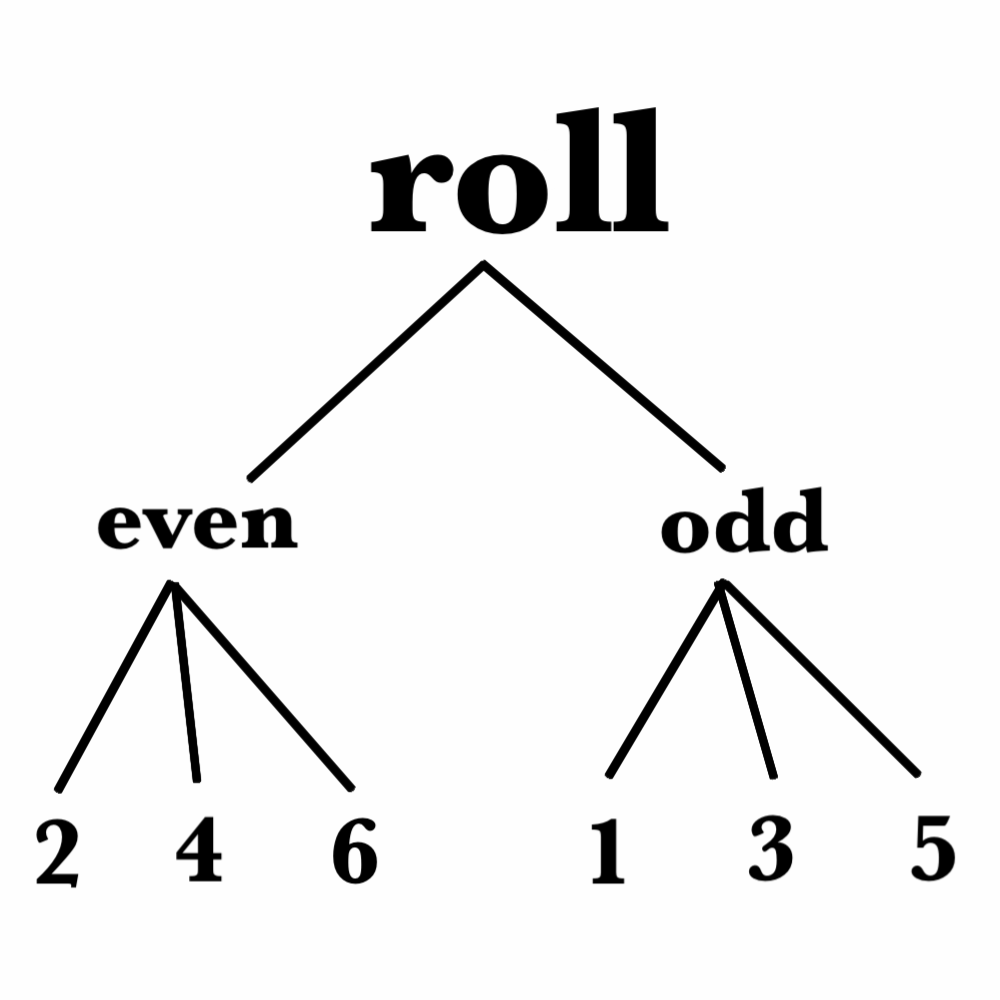
\includegraphics[width=.5\textwidth]{cond-prob.png}
\end{figure}
Note that at each stage the outcomes are equally likely.

\begin{exercise}
Use the decision tree to redo exercise 1.
\end{exercise}

\subsection*{Overlapping Events}
Let's consider the case of rolling a fair die with six sides.
Now suppose that we have the events $F$ which represents ``The die shows 1, 2, 3, or 5.'' and $E$ which represents ``The die shows an even number.''

What is the probability of "The die shows 1, 2, 3, or 5" ? Well, four of the outcomes are accounted for out of six total, so $\mathrm{Pr}(F) = 4/6$.

What is the probability that the roll shows an even number? Now three events are accounted for out of six, so $\mathrm{Pr}(E)=3/6$.


\begin{exercise}
Made a picture of the sample space in this case. Use two colors to indicate which outcomes are in the events $E$ and $F$.
\end{exercise}

\begin{exercise}
Use your diagram to compute the following two probabilities.
\begin{compactitem}
\item What is the probability that the die roll is even and "the die shows 1, 2, 3, or 5"?
\item What is the probability that the die roll is even, knowing that the die shows 1, 2, 3 or 5?
\end{compactitem}
\end{exercise}

\subsection*{Well-Shuffled Cards}
Consider the case where a magician draws one card from a well-shuffled standard pack of 52 cards. The magician will tell you if the card is either red or clubs, but not which. Call this information the event $R\cup C$, where $R$ represents the event of a red card and $C$ represents the event of a club. If you are told that the first card drawn is red or a club, then we know the event $R\cup C$ has occured.

\begin{exercise}
Draw a picture of the sample space in this situation, and use two colors to label the two events $R$ and $C$.

Use this diagram to find the probability of the event $R \cup C$.
\end{exercise}
\begin{exercise}
What is the probability that the card drawn is an ace?
\end{exercise}
\begin{exercise}
Use your sample space diagram to compute the following probabilities:
\begin{compactitem}
\item The card drawn is an Ace and is either red or a club.
\item The card drawn is an Ace if the magician tells you it is either red or a club.
\end{compactitem}
\end{exercise}


\subsection*{The Rule}

Looking at these examples, can you find a rule for computing conditional probabilities?
Think about it for a minute, and don't read on until you make a guess.

\vspace{1cm}

\hrule

\vspace{1cm}

To get things set out clearly, we need the idea of the intersection of two sets.

\begin{definition}
Let $A$ and $B$ be two sets.
The \emph{intersection} of these sets is the new set
\[
A \cap B = \{ x \mid \text{$x$ is an element of $A$ and $x$ is an elemenet of $B$.} \}
\]
which contains all those things which are elements of \textbf{both} sets.
\end{definition}



This notion of intersection is the word that corresponds to ``and'' when thinking about events.
This should be thought of as analogous to the word ``or'' and the union of two sets.


\begin{quotation}
Suppose that $A$ and $B$ are a pair of events.
Then the probability of $A$ given that you know $B$ has occured is given by the rule
\[
\mathrm{Pr}(A \mid B ) = \dfrac{ \mathrm{Pr}(A \cap B)}{\mathrm{Pr}(B)}.
\]
\end{quotation}

\begin{exercise}
Go back through the above examples and see how this rule is all that is happening.
All you have to do is change your perspective so that $B$, the given event, is your new sample space.
\end{exercise}


\subsection*{Challenge: The Monty Hall Problem}

In our first day of discussion about probability, we talked about the Monty Hall Problem.
The second decision in that set-up is really about conditional probability, because you are given extra relevant information.

\begin{challenge}
Use the notion of conditional probability to sort out why the best strategy is to change doors.
\end{challenge}

%\begin{thebibliography}{9}
%\end{thebibliography}

\end{document}
%sagemathcloud={"zoom_width":100}